% Owner: Hasan  |  Task: T8  |  Drafted by ORCA agents, finalised by the owner.
\section{Distillation Schemes}
\label{sec:schemes}

\textit{INTERPRETATION: the scheme-selection advice and cost/failure-mode comparisons are our synthesis; cited method descriptions and reported results are source-grounded.}

A training scheme specifies when the teacher exists, how many sources supervise the student, and what data the trainer can see. These choices affect compute and failure modes as much as the loss itself. A fixed offline teacher is convenient when it is already available; peer training removes the need for a privileged teacher but raises joint-training cost; teacher-free self-distillation avoids a second network but cannot add independent knowledge. Multi-teacher and assistant schemes trade compute for broader or better-matched guidance, while data-free methods trade access to original examples for synthetic-data quality and teacher-internal access.

\paragraph{Offline distillation.} The standard offline procedure trains a teacher first, freezes it, and then trains a student using labels and teacher outputs. Hinton et al. formulated softened class distributions as a target that complements ground truth. Later feature-based methods preserve this staged teacher/student arrangement while changing the transfer object: SimKD uses a projected penultimate feature with a reused frozen classifier, and FCFD routes student features through the teacher's later layers to test functional consistency\citep{hinton2015kd,chen2022simkd,liu2023fcfd}. CAT-KD transfers class-specific attention, while TCS builds a teacher-derived coordinate frame; both add intermediate or structured signals without requiring peer co-training\citep{guo2023catkd,zhou2025tcs}. These 2022--2025 inventory methods represent offline feature KD beyond the original logit objective.

Offline KD is a practical choice when a teacher checkpoint and the training data are available and training can be staged. It permits a larger teacher to be trained independently and makes student runs easy to reproduce from fixed targets, but the frozen teacher cannot adapt when the student exposes a mismatch. Materializing logits or features can reduce repeated teacher inference but costs storage; computing teacher outputs online saves storage but occupies accelerator time. A further limitation is that the scheme assumes the teacher can be accessed at all, including its intermediate layers for feature methods. If only outputs are available, logit KD or a method explicitly designed around outputs is more appropriate than hint matching or teacher-tail approaches. Offline training is therefore a reference arrangement, not a guarantee that teacher knowledge fits the student's capacity.

\paragraph{Online and mutual distillation.} Deep Mutual Learning (DML) established peer training in which each network learns from the others' current predictions, rather than receiving targets from a separately pretrained teacher. SwitOKD adds an adaptive switching threshold: a stronger peer may pause its expert role when the gap threatens to make guidance unhelpful. L-MCL adds mutual contrastive transfer between peer embeddings and meta-optimized layerwise knowledge exchange\citep{zhang2018dml,qian2022switokd,yang2023lmcl}. Both SwitOKD and L-MCL are 2022--2026 inventory methods. Relative to DML, SwitOKD directly controls when teacher-like peer supervision is emitted, while L-MCL enriches the signal beyond class probabilities; its extra layers and meta-optimization cost more machinery.

Online schemes fit settings where no fixed teacher exists, peer models can be trained together, and adaptive information exchange is useful. They avoid a separate teacher-pretraining stage and can let a weaker peer benefit from a stronger peer's evolving state. However, every participant must remain in the training graph, raising memory and compute with the number and size of peers. Early unstable predictions can be mutually reinforced; a lagging peer may transmit noise, and a dominant peer can make nominally mutual learning asymmetric in practice. SwitOKD's pause mechanism addresses teacher outrunning, while vanilla DML has no such explicit mode switch. L-MCL's richer contrastive and layerwise terms can help beyond logits but add tuning and representation-memory costs. Choose online KD when peers are available and the deployment target can be selected from jointly trained models; use a frozen offline teacher when training cost or memory makes simultaneous models impractical.

\paragraph{Self-distillation.} Self-distillation obtains targets from the same model, its internal branches, its training history, or its previous generation. BYOT teaches shallow classifiers from deeper sections of one network; Born-Again Neural Networks train a new same-architecture model from a prior generation's predictions. These are foundational examples, and their distinction is whether the teacher is an internal branch or a previously trained model\citep{zhang2019byot,furlanello2018bornagain}. Recent inventory methods include DLB, which reuses the previous mini-batch's predictions for overlapping examples, and USKD, which constructs customized soft labels without a separate pretrained teacher\citep{shen2022dlb,yang2023nkd}. DLB and USKD are 2022--2026 representatives. Compared with BYOT's multiple heads and Born-Again's repeated training rounds, DLB stores a limited prediction history and USKD derives targets from labels and predictions; these reduce external-teacher dependence but do not inject independent knowledge.

The inventory's ``label-averaging view'' refers to Jeong and Chung's 2025 theory paper, which analyzes multi-round self-distillation as label averaging and gives conditions for population accuracy under label noise, alongside partial-label refinement. It is a theory result, not a separate empirical training scheme, and the inventory leaf name should be reviewed by Hasan for a title that signals this status\citep{jeong2025selfdistill}. Self-distillation is attractive when model internals, prediction history, or an earlier generation are available but external teacher access is costly. It can regularize optimization without maintaining a second large model at inference, yet the signal is bounded by what that model already knows: confirmation bias can recycle its errors, and repeated generations can compound calibration or class-imbalance problems. BYOT is suitable when intermediate branches can be trained jointly; Born-Again fits repeated training budgets; DLB fits online reuse of recent examples; USKD fits label-available settings with no teacher. These choices differ in memory, sequential runtime, and how independent their target signal is.

\paragraph{Multi-teacher distillation.} With several pretrained teachers, Adaptive Ensemble KD combines teacher guidance in gradient space; the 2020 method is lineage for later multi-teacher approaches. MTKD-RL learns per-example teacher weights with a reinforcement-learning agent, and AGRE-KD selects teachers in relation to group-robust objectives. They are 2025 inventory methods that adapt teacher use beyond fixed averaging\citep{du2020aekd,yang2025mtkdrl,kenfack2025agrekd}. MTKD-RL compares teacher quality and teacher-student gaps per sample, whereas AGRE-KD uses agreement and group information to avoid a globally strong but biased source. Relative to equal-weight ensembles, both can reject or downweight unhelpful teachers; compared with gradient-space AE-KD, MTKD-RL introduces a learned policy and AGRE-KD targets worst-group behavior.

Multi-teacher schemes are useful when specialized teachers cover complementary classes, domains, or groups and no single teacher is uniformly best. They require access to multiple teacher checkpoints and their predictions or features, so training cost and memory usually rise with teacher count. Weighting can be unstable when teacher scores are noisy or teachers are redundant; a selector may also encode group imbalances from its data. Fixed averages are cheaper and easier to audit but can dilute a strong expert with a weak one. MTKD-RL is a fit when per-example teacher quality can be learned and the policy cost is acceptable; AGRE-KD is more appropriate when worst-group behavior is the target. If teacher diversity is low, the extra ensemble cost may not yield additional information, and a single adapted teacher or offline method is simpler.

\paragraph{Teacher assistants and capacity gap.} Cho et al. reported that a stronger or larger teacher does not always improve the student's result, challenging the assumption that teacher accuracy alone predicts transfer quality. This is a teacher-student compatibility problem, not proof that every large teacher fails; the original survey draft makes this same point with Cho's attribution, retained here\citep{cho2019efficacy}. Teacher Assistant KD (TAKD) inserts intermediate-capacity assistants between the original teacher and student, so each transfer crosses a smaller gap. It improves direct teacher-to-student matching when the endpoints differ greatly, but adds sequential training and checkpoint selection\citep{mirzadeh2020takd}.

Recent inventory methods alter the teacher signal rather than inserting a chain. ATS assigns separate temperatures to target and non-target logits to address large-teacher soft targets; DPK mixes teacher features as dynamic prior knowledge; AID adapts the teacher's intra-class distribution to the student\citep{li2022ats,qiu2023dpk,qian2025aid}. These methods are useful when the teacher is usable but its outputs or features are poorly matched to the student. Relative to TAKD, they avoid intermediate models but introduce method-specific choices: temperature asymmetry, feature masking, or teacher fine-tuning. ATS changes distribution sharpness with modest structural overhead; DPK needs feature access; AID spends compute adapting a teacher. Select TAKD when a capacity ladder is feasible and the gap is severe, or adaptation when a specific mismatch can be diagnosed and modifying the teacher is allowed. Failure can arise from an assistant that does not actually narrow the functional gap, or from adapting away information the student needs.

\paragraph{Data-free distillation.} Data-free KD addresses settings where training examples are unavailable or cannot be shared. DeepInversion is a foundational approach that synthesizes inputs by matching batch-normalization statistics of the teacher. NAYER changes the generation mechanism by using noisy layers and label-text embeddings instead of noisy input optimization; SSD-KD selects a small synthetic set according to difficulty and diversity. The 2024 NAYER and SSD-KD methods provide current inventory coverage\citep{yin2020deepinversion,tran2024nayer,liu2024ssdkd}. NAYER favors efficient generation, while SSD-KD explicitly trades some accuracy for fewer synthetic examples and lower training time relative to a larger-generation baseline.

Choose data-free KD when source data cannot be accessed but the teacher's parameters or internal statistics remain available. Unlike offline feature transfer on real examples, synthetic generation introduces another optimization or sampling process; synthetic inputs may cover teacher decision regions poorly, and batch-normalization assumptions fail for architectures without suitable statistics. SSD-KD's compact set reduces student training time but its inventory-reported CIFAR-100 result (75.16 in 4.22 hours) is below CMI's 77.04 in 15.42 hours in that paper's Table 2, illustrating an explicit efficiency-accuracy trade-off rather than universal superiority. % src: SSD-KD Table 2
NAYER reports 77.54 on CIFAR-100 ResNet-34 to ResNet-18 in Table 1, but this result must be interpreted under the paper's data-free protocol and not compared directly with methods using original training data. % src: NAYER Table 1
Data-free schemes can therefore preserve privacy or enable transfer across data boundaries, but they do not remove the need for teacher access, and synthetic coverage is their central failure mode.

\subsection{Scheme-level comparison}

Table~\ref{tab:scheme-comparison} summarizes resource assumptions and representative methods. It treats ``teacher needed'' as a pretrained external model, distinguishing that from peers or internal branches that act as teachers during training. Cost labels are qualitative because the inventory does not report comparable FLOPs or memory for every method.

\begin{table*}[t]
\centering\small
\begin{tabular}{p{2.2cm}p{2.6cm}p{3.2cm}p{5.1cm}}
\toprule
Scheme & Pretrained external teacher? & Extra training cost & Representative methods (registry IDs) \\
\midrule
Offline & Yes & Teacher training/inference staged; fixed targets may be cached & SimKD (\texttt{chen2022simkd}), FCFD (\texttt{liu2023fcfd}), CAT-KD (\texttt{guo2023catkd}), TCS (\texttt{zhou2025tcs}) \\
Online / mutual & No & Jointly hold and update multiple peers; cost scales with peers & SwitOKD (\texttt{qian2022switokd}), L-MCL (\texttt{yang2023lmcl}) \\
Self-distillation & No separate model; internal/previous teacher signal & Extra branches, prediction history, or sequential generations & DLB (\texttt{shen2022dlb}), USKD (\texttt{yang2023nkd}) \\
Multi-teacher & Yes, multiple & Teacher inference and selection/weighting overhead & MTKD-RL (\texttt{yang2025mtkdrl}), AGRE-KD (\texttt{kenfack2025agrekd}) \\
Assistant / gap adaptation & Yes & Assistant chain or teacher adaptation; feature methods need teacher internals & ATS (\texttt{li2022ats}), DPK (\texttt{qiu2023dpk}), AID (\texttt{qian2025aid}) \\
Data-free & Yes, model access needed & Synthetic generation plus student training; no original data pass & NAYER (\texttt{tran2024nayer}), SSD-KD (\texttt{liu2024ssdkd}) \\
\bottomrule
\end{tabular}
\caption{Qualitative scheme comparison. Actual runtime and memory depend on architecture, batch size, implementation, and whether teacher outputs are cached.}\label{tab:scheme-comparison}
\end{table*}

No scheme dominates all settings. Offline transfer minimizes coordination but cannot adapt the teacher; online transfer adapts peers at higher simultaneous compute; self-distillation saves external-teacher access while reusing correlated predictions. Multi-teacher training adds coverage at the cost of storage and selection complexity, whereas assistant chains or adapted teachers target a capacity mismatch more directly. Data-free KD is distinguished by data access rather than teacher count and still pays for synthesis. Choosing among them should follow the constraint that motivates KD: unavailable teacher, excessive capacity gap, privacy restrictions, compute budget, or lack of a single reliable teacher. Once the scheme is selected, the type of transferred knowledge and the way its gradients interact with labels remain independent choices addressed in Sections III and VI.

% Fig. 4: Scheme comparison by source of guidance and training arrangement.
\begin{figure}[t]
\centering
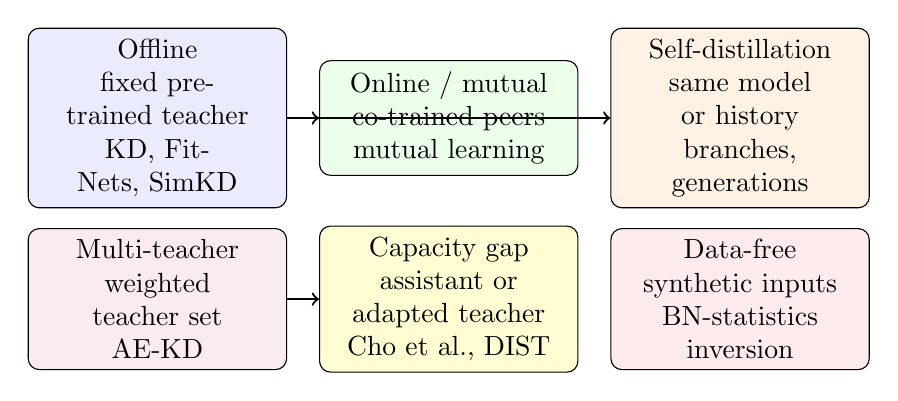
\begin{tikzpicture}[box/.style={draw,rounded corners,align=center,text width=3.0cm,minimum height=1.45cm,inner sep=4pt}, arr/.style={->,thick}]
\node[box,fill=blue!8] (offline) at (0,0) {Offline\\fixed pretrained teacher\\KD, FitNets, SimKD};
\node[box,fill=green!8] (online) at (3.7,0) {Online / mutual\\co-trained peers\\mutual learning};
\node[box,fill=orange!10] (self) at (7.4,0) {Self-distillation\\same model or history\\branches, generations};
\node[box,fill=purple!8] (multi) at (0,-2.3) {Multi-teacher\\weighted teacher set\\AE-KD};
\node[box,fill=yellow!18] (gap) at (3.7,-2.3) {Capacity gap\\assistant or adapted teacher\\Cho et al., DIST};
\node[box,fill=red!8] (free) at (7.4,-2.3) {Data-free\\synthetic inputs\\BN-statistics inversion};
\draw[arr] (offline) -- (online);
\draw[arr] (offline) -- (self);
\draw[arr] (multi) -- (gap);
\end{tikzpicture}
\caption{Training schemes differ in teacher availability, number of guidance sources, and whether original training data are available. Arrows indicate alternative arrangements, not a required progression.}
\label{fig:schemes}
\end{figure}

